\documentclass[notitlepage]{article}
\usepackage{amsmath}
\usepackage{mathtools}
\usepackage{amsthm}
\usepackage{amssymb}
\usepackage{graphicx}
\usepackage{array}
\usepackage{wrapfig}
\usepackage{algorithm}% http://ctan.org/pkg/algorithm
% \usepackage{algorithmic}
\usepackage{algpseudocode}% http://ctan.org/pkg/algorithmicx
\usepackage[utf8]{inputenc}
\usepackage[a4paper, margin=2.5cm, left=3.5cm, right=3.5cm]{geometry}
\usepackage{accents}
\usepackage{float}
\usepackage{hyperref}
\usepackage{bookmark}
\usepackage{multirow}
\usepackage{pdfpages}
\usepackage{subcaption}
\usepackage{sectsty}
\usepackage{ragged2e}
\usepackage{titlesec}
\usepackage{listings}
\usepackage{etoolbox}
\usepackage[outline]{contour}
\usepackage[font=small,skip=1pt]{caption}
\usepackage{enumitem}
\usepackage{tikz}
%Includes "References" in the table of contents
\usepackage[nottoc]{tocbibind}
\usepackage{appendix}
\usepackage{xcolor,colortbl}


\newcommand{\highlight}[1]{{\cellcolor{yellow!30} #1}}

\setlength\parindent{0pt}

\setlength{\tabcolsep}{20pt}
\renewcommand{\arraystretch}{1.5}

\newcolumntype{P}[1]{>{\centering\arraybackslash}p{#1}}
\newcolumntype{M}[1]{>{\centering\arraybackslash}m{#1}}

\algnewcommand\algorithmicforeach{\textbf{for each}}
\algdef{S}[FOR]{ForEach}[1]{\algorithmicforeach\ #1\ \algorithmicdo}

\titleformat{\chapter}[block]
  {\normalfont\huge\bfseries}{\thechapter.}{10pt}{\huge}
\titlespacing*{\chapter}{0pt}{0pt}{10pt}

\makeatletter
\patchcmd{\chapter}{\if@openright\cleardoublepage\else\clearpage\fi}{}{}{}
\makeatother

\title{Parallel Boruvka\\{\normalsize Final project for the SPM course 2020/21}}
\author{Matteo De Francesco}
\date{}

\begin{document}

\maketitle

\thispagestyle{empty}

\tableofcontents

\newpage

\pagenumbering{arabic}

\section{Introduction}

In this report we will analyze a parallel implementation of the Boruvka algorithm.\\
Boruvka algorithm is used to discover the {\bf MST} (\textit{Minimum Spanning Tree}) of a given graph. It proceeds in the following way:

\begin{algorithm}[H]
  \caption{Boruvka Algorithm}
  \begin{algorithmic}[1]
    \Function{Boruvka Algorithm}{$V, E$}
      \State $Comp = \left[\,\right]$\Comment{Initialize empty components}
      \ForEach{$v \in V$}
        \State add $v$ to $Comp$\Comment{Add each vertex to the Components}
      \EndFor
      \State $MST = \left\{\,\right\}$\Comment{Initialize empty MST}
      \While{$|Comp| > 1$}\Comment{Until there is more than one component left}
        \ForEach{$c \in Comp$} \label{alglin:foreach}
          \State $E' =$ \texttt{getMinEdges}($c, V, E$)
          \State add $\min e \in E'$ to $MST$
        \EndFor
        \State Merge components \label{alglin:merge}
      \EndWhile
      \State \Return $MST$
    \EndFunction
  \end{algorithmic}
\end{algorithm}

and the function \texttt{getMinEdges} does the following

\begin{algorithm}[H]
  \caption{Get min edges function}
  \begin{algorithmic}[1]
    \Function{getMinEdges}{$c, V, E$}
      \State $E_{tot} = \left[\,\right]$
      \ForEach{$v \in c.vertices$}\Comment{Iterate through all the vertices in the component}
        \State $E'$ = Find all edges involving $v$\Comment{Find all edges where $v$ is present}
        \State $e.val = +Inf$\Comment{Minimum node found, set starting value to $\infty$}
        \ForEach{$e' \in E'$}
          \State \# Check if $v$ is not linked to another $v$ in the same component
          \If{$e'.destNode \notin c.vertices$ and $e'.val < e.val$}
            \State $e = e'$\Comment{Update $e$}
          \EndIf
        \EndFor
        \State Add $e$ to $E_{tot}$
      \EndFor
      \State \Return $E_{tot}$
    \EndFunction
  \end{algorithmic}
\end{algorithm}

Basically the algorithm starts by initializing each component with a vertex. For each component, the algorithm look for the minimum edge that links it with a different component, and update the $MST$ with it.\\
After the minimum edges are found, the algorithm merge the components together based on the edges present in the $MST$. When the component is composed by more than one vertex, we look for the minimum edge by 
repeating the procedure on each node in the component, always satisfying the condition that the other node must not be in the same component (otherwise we create a cycle).\\
This is repeated until there is only one component left, which is the desired minimum spanning tree.

\section{Parallel Implementation}

As we can see from the above algorithm, the code can be easily parallelized with a \texttt{map-reduce} approach.\\
Indeed, the line \ref{alglin:foreach} can be easily parallelized by distributing the components among the different computational resources we have, each one computing the same function
(which coincide with the loop body).
Then, in the line \ref{alglin:merge}, a \texttt{reduce} approach can be used to merge the components using the selected edges in $MST$.\\
We can notice also how there is no condition when for each component we add the minimum edge to the $MST$ (two components can add also the same edge, which is exactly the link between the two components). 
This implies that we have no need for synchronization over the $MST$. However, since each thread will execute on a different core, we can assume that each cache level of each core will store  
the global variable $MST$. If we keep it global, we don't need synchronization among threads, but the cache coherency protocol need to update $MST$ in each cache whenever this is modified by a thread.\\
A better solution is to keep a local copy of $MST$ per each thread and at the end merge them all together in the global $MST$.\\
A possible schema of our parallel application can be the following:

\begin{figure}[H]
  \centering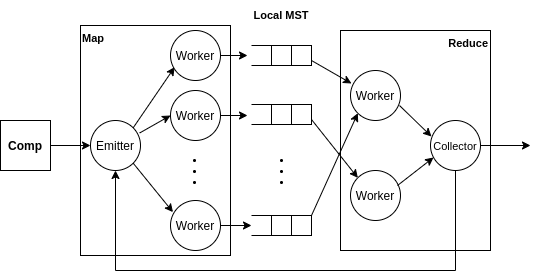
\includegraphics[scale=0.7]{pics/parallel_schema.png}
\end{figure}

As components arrives, the {\itshape Emitter} splits the workload among different workers. Each worker apply the map function and create a local copy of $MST$, which is stored in the queue. As soon as 
all the components are processed, the {\itshape reduce} part begins and the different edges in the local $MST$ are connected together. In this way we update the global $MST$ and obtain new components, 
which are sent back from the {\itshape Collector} to the {\itshape Emitter} and the cycle repeats, until there is only one component left.

\end{document}